


\documentclass[14pt,a4paper]{extarticle}

\usepackage[utf8]{inputenc}
\usepackage[T2A]{fontenc}
\usepackage{amssymb,amsmath,mathrsfs,amsthm}
\usepackage[russian]{babel}
\usepackage{graphicx}
\usepackage[footnotesize]{caption2}
\usepackage{indentfirst}
\usepackage{multicol}
\usepackage{listings}
\usepackage{float}
\usepackage{url}

\usepackage{enumitem}

%\usepackage[ruled,section]{algorithm}
%\usepackage[noend]{algorithmic}
%\usepackage[all]{xy}
\usepackage{booktabs}
\usepackage{graphicx}
\usepackage[table,xcdraw]{xcolor}
\usepackage{tcolorbox}

%Библиотека для блок-схем
\usepackage{tikz}
\usetikzlibrary{shapes,arrows}

% Параметры страницы
\textheight=24cm
\textwidth=16cm
\oddsidemargin=5mm
\evensidemargin=-5mm
\marginparwidth=36pt
\topmargin=-1cm
\footnotesep=3ex
%\flushbottom
\raggedbottom
\tolerance 3000
% подавить эффект "висячих стpок"
\clubpenalty=10000
\widowpenalty=10000
%\renewcommand{\baselinestretch}{1.1}
\renewcommand{\baselinestretch}{1.5} %для печати с большим интервалом

\newtheorem{definition}{Определение} % задаём выводимое слово (для определений)
\newtheorem{example}{Пример} % задаём выводимое слово (для определений)
\newtheorem{construction}{Конструкция} % задаём выводимое слово (для определений)
\newtheorem{theorem}{Теорема} % задаём выводимое слово (для определений)



\begin{document}
\begin{titlepage}


\begin{center}
%\ \vspace{-2cm}



%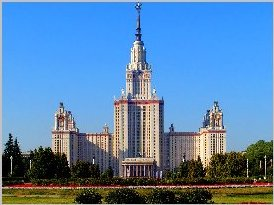
\includegraphics[width=0.5\textwidth]{msu.eps}\\
{Московский государственный университет имени М.В.~Ломоносова}\\
Механико-математический факультет\\
%Кафедра Вычислительной математики
\ \vspace{+2cm}


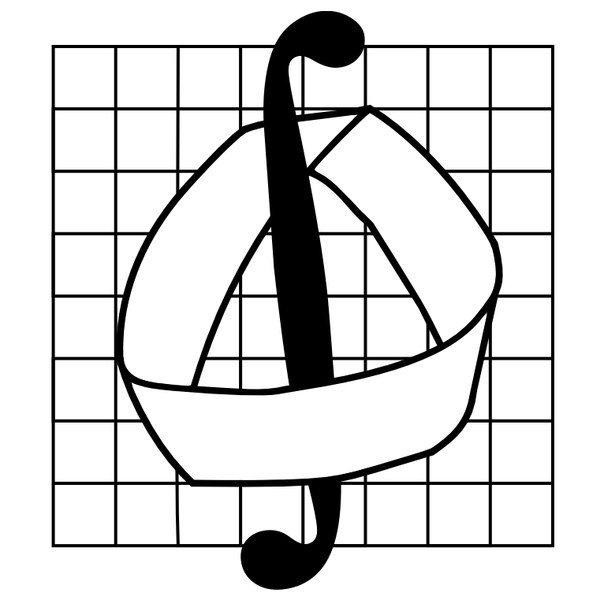
\includegraphics[width=0.3\textwidth]{mehmat.jpg}\\


\vspace{1cm}

{\large РЕФЕРАТ}

{\Large\bfseries
Рабочее время и время отдыха
\\}
{\large Сибгатуллин Артур, 610 группа}

\end{center}

\vspace{1cm}

\vspace{7cm}

\begin{center}
Москва, 2023
\end{center}


\enlargethispage{4\baselineskip}
\end{titlepage}

\newpage
\renewcommand{\contentsname}{Содержание}
\tableofcontents
\newpage



\section{Отпуска, их виды. Порядок предоставления отпусков}
Работники имеют право на трудовые и социальные отпуска при наличии оснований, предусмотренных законодательством.

\textbf{Отпуск} - освобождение от работы по трудовому договору на определенный период для отдыха и иных социальных целей с сохранением прежней работы и заработной платы.

Отпуска подразделяются на два вида:\
\begin{itemize}
	\item \textbf{Трудовые}. К трудовым отпускам относятся: основной минимальный отпуск; основной удлиненный отпуск; дополнительные отпуска.
	\item \textbf{Социальные}. К социальным отпускам относятся: отпуск по беременности и родам; в связи с обучением без отрыва от производства; в связи с катастрофой на ЧАЭС; творческие; по уважительным причинам личного и семейного характера.
\end{itemize}

Трудовой отпуск предоставляется ежегодно за работу в течение года (за рабочий год). Рабочий год, за который предоставляется трудовой отпуск - это промежуток времени, равный продолжительности календарному году, но исчисляемый для каждого работника со дня приема на работу и продолжающийся до такой же даты следующего года.

Продолжительность отпуска исчисляется в календарных днях. В число календарных дней любого отпуска не включаются и не оплачиваются государственные праздники и праздничные дни, приходящиеся на время отпуска.

Отпуска оформляются приказом (распоряжением) нанимателя или запиской об отпуске, которые подписываются от имени нанимателя уполномоченным или должностным лицом нанимателя.

Кодексом установлено, что работники имеют право на отпуск независимо от того, кто является их нанимателем, какова форма организации, и каков вид трудового договора с ними заключен, какова оплата его труда. Совместители, временные работники имеют также право на отпуск.

Закон различает основной минимальный отпуск и основной удлиненный отпуск.

Дополнительные отпуска. Дополнительные отпуска предоставляются лишь некоторым категориям работников в связи с особыми условиями или характером труда либо в качестве поощрения за длительную непрерывную работу на одном предприятии.

Дополнительные отпуска за работу с вредными условиями труда, за ненормированный рабочий день, за продолжительный стаж работы в одной организации. За счет собственных средств наниматель может предоставлять дополнительные поощрительные отпуска.

\subsection{Трудовые отпуска}
Право на первый ежегодный оплачиваемый отпуск возникает у работников по истечении шести месяцев работы у данного нанимателя. Для отдельных категорий работников наниматель обязан по их требованию предоставить им отпуск до истечения шестимесячного срока работы. К таким лицам относятся: женщины - перед отпуском по беременности и родам или после него; лица моложе 18 лет; работники, принятые на работу в порядке перевода; другие категории работников в соответствии с законодательством.

Трудовые отпуска (основной и дополнительный) за второй и последующие рабочие годы предоставляются в любое время рабочего года в соответствии с очередностью предоставления трудовых отпусков.

Ежегодный трудовой отпуск предоставляется за каждый рабочий год, который начинается со дня истечения предыдущего рабочего года. За второй и последующие годы отпуск может предоставляться и авансом. Однако и в этом случае он предоставляется и оплачивается в полном размере, а не пропорционально отработанному времени.

При составлении графиков должны учитываться требования законодательства о предоставлении отпусков отдельным категориям работников в летнее или удобное время или во время, определенное законом.

Дата начала трудового отпуска определяется по договоренности между работником и нанимателем. Как правило, с целью обеспечения нормальной деятельности предприятия отпуска должны распределяться равномерно в течение месяца.

Наниматель обязан уведомить работника о времени начала трудового отпуска не позднее чем за 15 дней. Отпуск оформляется приказом (распоряжением) нанимателя или запиской об отпуске. По просьбе работника наниматель может изменить время начала отпуска, предусмотренного в графике.

Наниматель обязан предоставить работнику отпуск как правило, в течение каждого рабочего года.

Работникам моложе 18 лет и работникам, имеющим право на дополнительный отпуск в связи с вредными условиями труда запрещается непредоставление трудового отпуска.

Наниматель обязан выплатить средний заработок за время трудового отпуска не позднее чем за два дня до начала отпуска.

В определенных законом случаях работник имеет право на перенос или продление трудового отпуска:
\begin{enumerate}
\item при временной нетрудоспособности работника;
\item при наступлении срока отпуска по беременности и родам;
\item в случае привлечения работника к выполнению государственных обязанностей с правом на освобождение от работы;
\item при совпадении трудового отпуска с отпуском в связи с обучением (если работник оформил такой отпуск перед трудовым отпуском или во время последнего после получения вызова учебного заведения);
\item в случаях невыплаты работнику в установленный срок заработной платы за время отпуска;
\item с согласия сторон, а также в других случаях, предусмотренных законодательством или коллективным договором. об отзыве работника из трудового отпуска с указанием об условиях использования оставшейся части отпуска.
\end{enumerate}

Не допускается отзыв из отпуска работников моложе 18 лет, и работников, занятых на работах с вредными условиями труда. Запрещается перенос дополнительного отпуска за работу во вредных условиях труда на следующий год или замена его денежной компенсацией.


\subsection{Социальные отпуска}.

Социальные отпуска предоставляются работникам в целях создания благоприятных условий для материнства, ухода за детьми, образования без отрыва от производства, удовлетворения семейно-бытовых потребностей и для других социальных целей.

В отличие от трудового отпуска социальные отпуска:
\begin{itemize}
	\item предоставляются не для отдыха, а для других признаваемых общественно-полезными (социальных) целей;
	\item право на социальные отпуска не зависит от продолжительности, места и вида работы;
	\item заработная плата за время социальных отпусков сохраняется в случаях, предусмотренных в ТК или коллективным договором, соглашением;
	\item все социальные отпуска являются самостоятельным видом отпуска. Они предоставляются сверх трудового отпуска вместе с ним или отдельно от него;
	\item социальные отпуска предоставляются не за рабочий, а за календарный год, причем только за тот, в котором работник имеет на них право. Если в текущем календарном году социальный отпуск не использован, то на следующий год он не переносится и денежной компенсацией, в том числе и при увольнении, не заменяется.
\end{itemize}


К социальным отпускам относятся:
\begin{itemize}
	\item по беременности и родам;
	\item в связи с катастрофой на Чернобыльской АЭС;
	\item по уважительным причинам личного и семейного характера
\end{itemize}


\section{Больничные}
Больничные регулируются Федеральным законом «Об обязательном социальном страховании на случай временной нетрудоспособности и в связи с материнством» и отдельными статьями ТК РФ. 

Согласно законодательству, «листок нетрудоспособности» подтверждает, что работник болеет и ему положена компенсация, которая оплачивается из Фонда социального страхования, где лежат отчисления с заработной платы сотрудника. 

Примеры ситуаций, при которых оформляется больничный:
\begin{itemize}
	\item болезнь (травма) гражданина;
	\item долечивание работника в санаторно-курортном учреждении;
	\item протезирование в стационаре;
	\item болезнь члена семьи, за которым необходим уход;
	\item беременность и предстоящие роды;
	\item карантин.
\end{itemize}

\subsection {Выплаты}

Когда больничный выплачивается в связи с болезнью или травмой сотрудника:
\begin{itemize}
	\item за первые три дня выплаты идут из средств работодателя (страхователя);
	\item за последующие дни — из средств Фонда социального страхования России.
\end{itemize}


В иных случаях — уход за больным членом семьи, карантин, протезирование, долечивание в санатории — пособие выплачивается за счет средств ФСС с первого дня.


Размер выплат зависит от стажа и среднего заработка:
\begin{itemize}
	\item менее пяти лет — выплаты составят $60\%$ от среднего заработка;
	\item от пяти до восьми лет — $80\%$ среднего заработка; 
	\item более восьми — $100\%$ среднего заработка. 
\end{itemize}


Стаж высчитывается по трудовой книжке, договорам, справкам или сведениям о перечисленной заработной плате из ПФР. Для расчета среднего заработка берут все выплаты, на которые уплачивались страховые взносы за последние два года, в том числе у предыдущего работодателя.

Больничный лист выдается медицинскими организациями, уполномоченными на экспертизу временной нетрудоспособности. Это могут быть в том числе частные клиники с подходящей лицензией. Пособие выплачивается за календарные дни, то есть за весь период, на который выдан листок нетрудоспособности.

Также существует максимум пособия. При любом размере зарплаты пособие по нетрудоспособности за день не превысит установленный лимит. Однако каждый год он увеличивается. Максимальная оплата больничного листа поставлена в зависимость от предельной величины базы для начисления страховых взносов в ФСС. В 2018 году она составила 815 000 рублей, в 2019 году — 865 000 рублей, в 2020 году — 912 000 рублей, в 2021 году — 966 000 рублей.

При расчете среднего дневного заработка учитываются выплаты за два года до года начала болезни. Так, в 2021 году значение среднедневного заработка для расчета максимальной выплаты по больничному составит не больше: (865 000 + 912 000) / 730 [дней] = 2 434,24 рублей.

Cо дня нарушения пособие будут считать из МРОТ. Если причиной болезни сотрудника стало алкогольное, наркотическое или токсическое опьянение, то пособие за весь период болезни считают из МРОТ. Пособие по временной нетрудоспособности при утрате трудоспособности вследствие заболевания или травмы выплачивается за весь период до дня восстановления трудоспособности или установления инвалидности.

Если по истечении 15-дневного срока пациенту не стало лучше, то для продления больничного потребуется медкомиссия. Если по медицинским показаниям больной должен лечь в стационар, то больничный оформляется на весь срок нахождения в лечебном учреждении. После этого врач больницы может продлить документ на 10 дней для реабилитации в домашних условиях. В случае длительного лечения медорганизация выдает новый листок нетрудоспособности и одновременно оформляет предыдущий листок нетрудоспособности для назначения и выплаты пособия по временной нетрудоспособности, беременности и родам.

Больничный по уходу за ребенком можно продлевать до его полного выздоровления только если ребенку меньше семи лет.

Не допускается увольнение работника по инициативе работодателя (за исключением случая ликвидации организации или прекращения деятельности ИП) в период его временной нетрудоспособности и в период пребывания в отпуске.


\addcontentsline{toc}{section}{\protect\numberline{}Список литературы}%
\begin{thebibliography}{3}


\bibitem{Belov} Правоведение : учебник для бакалавриата и специалитета / В. А. Белов [и др.] ; под редакцией В. А. Белова, Е. А. Абросимовой. — 4-е изд., перераб. и доп. — Москва : Издательство Юрайт, 2019. — 414 с. — (Бакалавр и специалист). — ISBN 978-5-534-06229-8. — Текст : электронный // Образовательная платформа Юрайт [сайт]. — URL: https://urait.ru/bcode/441662 (дата обращения: 22.11.2023). 


\bibitem{tk_rf} Трудовой кодекс Российской Федерации от 30 декабря 2001 г. N 197-ФЗ (ред. от 4 августа 2023 г.)

\end{thebibliography}


%\bibliographystyle{ugost2003s}
%\bibliography{biblio}



\end{document}
